\title{คาบเรียนที่ 1: พีชคณิตของเวกเตอร์ ขนาดของเวกเตอร์ และผลคูณจุด}
\frame{\titlepage}

\begin{frame}{สารบัญ}
\tableofcontents
\end{frame}

%%%%%%%%%%%%%
\section{พีชคณิตเวกเตอร์}
\frame{\sectionpage}
%%%%%%%%%%%%%

\begin{frame}
\frametitle{เวกเตอร์คืออะไร?}
\addfig{0.8}{vector_intro_image}{\href{https://www.youtube.com/watch?v=fNk_zzaMoSs&ab_channel=3Blue1Brown}{Vectors | Chapter 1, Essence of linear algebra}}{}
\end{frame}

\begin{frame}
\frametitle{การเขียนเวกเตอร์}
\begin{defn}{}{}
\begin{itemize}
\item เวกเตอร์ 2 มิติ: $\vec{v} = \langle v_1, v_2 \rangle$ โดยที่ $v_1, v_2$ เป็นจำนวนจริง \pa
\item เวกเตอร์ 3 มิติ: $\vec{v} = \langle v_1, v_2, v_3 \rangle$  โดยที่ $v_1, v_2, v_3$ เป็นจำนวนจริง 
\end{itemize}
\end{defn}
\end{frame}

\begin{frame}
\begin{figure}[h!]
\centering
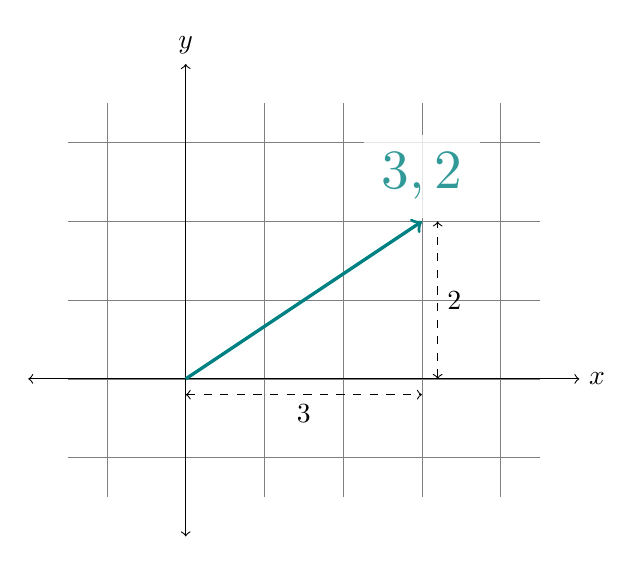
\begin{tikzpicture}
\draw[gray, very thin] (-1.5,-1.5) grid (4.5,3.5);
\draw[<->] (-2,0) -- (5,0) node [pos=1, right] {$x$};
\draw[<->] (0,-2) -- (0,4) node [pos=1, above] {$y$};
\draw[->, very thick, teal] (0,0) -- (3,2) node [fill = white, fill opacity = 0.8, pos=1, above, scale = 2] {$\bv{\red{3},\blue{2}}$};
\draw[<->, dashed] (0,-0.2) -- (3,-0.2) node [pos = 0.5, below] {$\red{3}$};
\draw[<->, dashed] (3.2,0) -- (3.2,2) node [pos = 0.5, right] {$\blue{2}$};
\end{tikzpicture}
\caption{เวกเตอร์ $\bv{3,2}$}
\end{figure}
\end{frame}

\begin{frame}
\begin{figure}[h!]
\centering
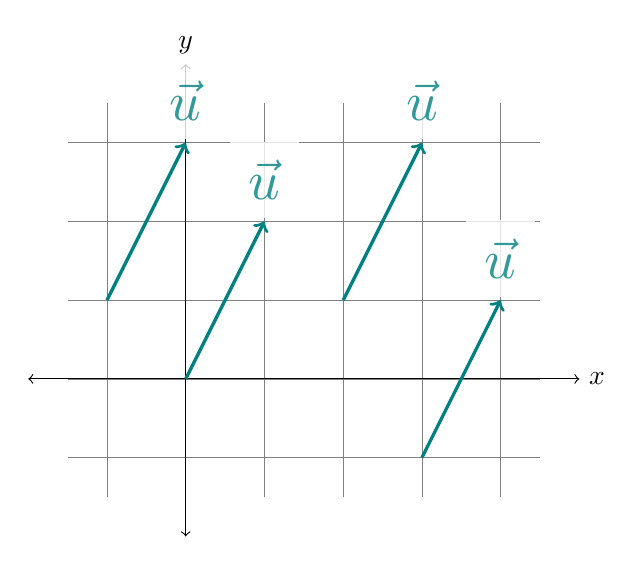
\begin{tikzpicture}
\draw[gray, very thin] (-1.5,-1.5) grid (4.5,3.5);
\draw[<->] (-2,0) -- (5,0) node [pos=1, right] {$x$};
\draw[<->] (0,-2) -- (0,4) node [pos=1, above] {$y$};
\draw[->, very thick, teal] (-1,1) -- (0,3) node [fill = white, fill opacity = 0.8, pos=1, above, scale = 2] {$\vec{u}$};
\draw[->, very thick, teal] (0,0) -- (1,2) node [fill = white, fill opacity = 0.8, pos=1, above, scale = 2] {$\vec{u}$};
\draw[->, very thick, teal] (3,-1) -- (4,1) node [fill = white, fill opacity = 0.8, pos=1, above, scale = 2] {$\vec{u}$};
\draw[->, very thick, teal] (2,1) -- (3,3) node [fill = white, fill opacity = 0.8, pos=1, above, scale = 2] {$\vec{u}$};
\end{tikzpicture}
\caption{เวกเตอร์ $\vec{u}$ มีค่าเท่าเดิม ไม่ว่าจะมีจุดเริ่มต้นที่ใดก็ตาม}
\end{figure}
\end{frame}

\begin{frame}
\begin{figure}[h!]
\centering
\begin{tikzpicture}
\draw[<->] (0,0) -- (5,0) node [right] {$x$};
\draw[<->] (0,0) -- (-2,-2) node [below left] {$y$};
\draw[<->] (0,0) -- (0,3) node [below left] {$z$};
\draw[->, very thick] (0,0) -- (2.59,1.59) node [above, scale = 2] {$\bv{\red{4},\blue{2},\color{teal}{3}}$};
\draw[->, dashed, red] (0,0) -- (4,0) node [pos = 0.3, below] {4};
\draw[->, dashed, blue] (4,0) -- (2.59,-1.41) node [pos = 0.5, below right] {2};
\draw[->, dashed, teal] (2.59,-1.41) -- (2.59, 1.59) node [pos = 0.8, right] {3};
\end{tikzpicture}
\caption{เวกเตอร์ $\bv{4,2,3}$}
\end{figure}
\end{frame}

\begin{frame}
\frametitle{เวกเตอร์เชิงเรขาคณิต}
\begin{defn}{พีชคณิตของเวกเตอร์ในปริภูมิสองมิติ}{}
ถ้า $\vec{u} = \langle u_1, u_2 \rangle, \pa \vec{v} = \langle v_1, v_2 \rangle$ \pa เป็นเวกเตอร์ และ $k$ เป็นจำนวนจริงแล้ว \pa
\begin{itemize}
\item $\vec{u} + \vec{v} = \bv{u_1+v_1, u_2+v_2}$ \pa
\item $\vec{u} - \vec{v} = \bv{u_1 - v_1, u_2 - v_2} $ \pa
\item $k \vec{u} = \bv{ku_1, ku_2}$
\end{itemize}
\end{defn}
\end{frame}

\begin{frame}
\begin{figure}[h!]
\centering
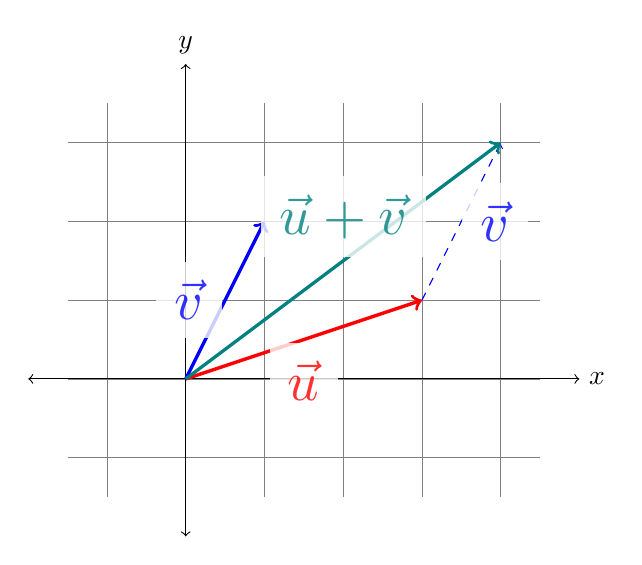
\begin{tikzpicture}
\draw[gray, very thin] (-1.5,-1.5) grid (4.5,3.5);
\draw[<->] (-2,0) -- (5,0) node [pos=1, right] {$x$};
\draw[<->] (0,-2) -- (0,4) node [pos=1, above] {$y$};
\draw[->, very thick, red] (0,0) -- (3,1) node [fill = white, fill opacity = 0.8, pos=0.5, below, scale = 2] {$\vec{u}$};
\draw[->, very thick, blue] (0,0) -- (1,2) node [fill = white, fill opacity = 0.8, pos=0.5, left, scale = 2] {$\vec{v}$};
\draw[->, dashed, blue] (3,1) -- (4,3) node [fill = white, fill opacity = 0.8, pos=0.5, right, scale = 2] {$\vec{v}$};
\draw[->, very thick, teal] (0,0) -- (4,3) node [fill = white, fill opacity = 0.8, pos=0.5, above, scale = 2] {$\vec{u} + \vec{v}$};
\end{tikzpicture}
\caption{ผลบวกเวกเตอร์ $\vec{u} + \vec{v}$}
\end{figure}
\end{frame}

\begin{frame}
\begin{figure}[h!]
\centering
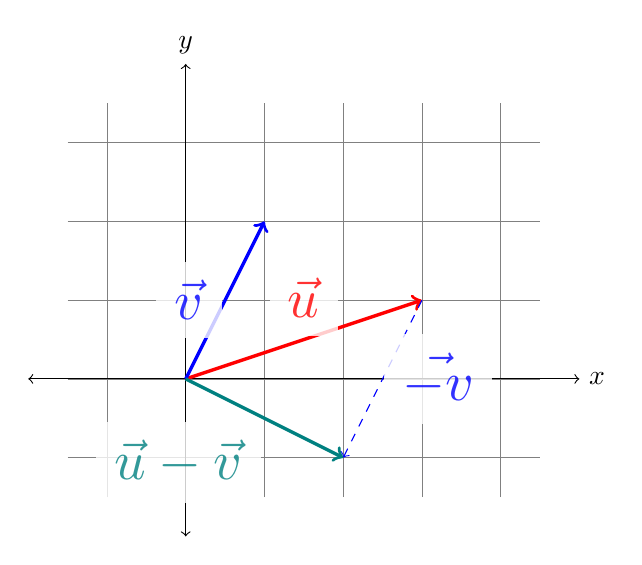
\begin{tikzpicture}
\draw[gray, very thin] (-1.5,-1.5) grid (4.5,3.5);
\draw[<->] (-2,0) -- (5,0) node [pos=1, right] {$x$};
\draw[<->] (0,-2) -- (0,4) node [pos=1, above] {$y$};
\draw[->, very thick, red] (0,0) -- (3,1) node [fill = white, fill opacity = 0.8, pos=0.5, above, scale = 2] {$\vec{u}$};
\draw[->, very thick, blue] (0,0) -- (1,2) node [fill = white, fill opacity = 0.8, pos=0.5, left, scale = 2] {$\vec{v}$};
\draw[->, dashed, blue] (3,1) -- (2,-1) node [fill = white, fill opacity = 0.8, pos=0.5, right, scale = 2] {$\vec{-v}$};
\draw[->, very thick, teal] (0,0) -- (2,-1) node [fill = white, fill opacity = 0.8, pos=0.5, below left, scale = 2] {$\vec{u} - \vec{v}$};
\end{tikzpicture}
\caption{ผลลบเวกเตอร์ $\vec{u} - \vec{v}$}
\end{figure}
\end{frame}

\begin{frame}
\begin{figure}[h!]
\centering
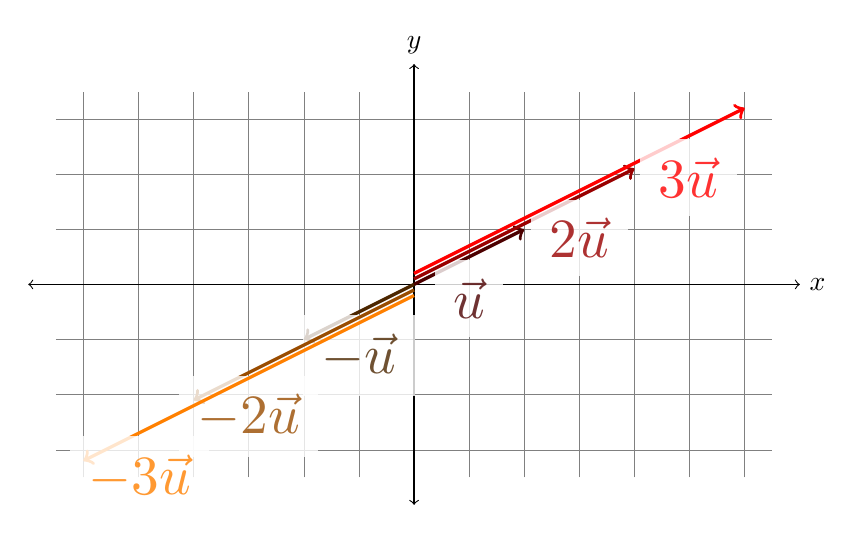
\begin{tikzpicture}[scale =0.7]
\draw[gray, very thin] (-6.5,-3.5) grid (6.5,3.5);
\draw[<->] (-7,0) -- (7,0) node [pos=1, right] {$x$};
\draw[<->] (0,-4) -- (0,4) node [pos=1, above] {$y$};
\draw[->, very thick, red!30!black] (0,0) -- (2,1) node [fill = white, fill opacity = 0.8, pos=0.5, below, scale = 2] {$\vec{u}$};
\draw[->, very thick, red!60!black] (0,0.1) -- (4,2.1) node [fill = white, fill opacity = 0.8, pos=0.75, below, scale = 2] {$2\vec{u}$};
\draw[->, very thick, red] (0,0.2) -- (6,3.2) node [fill = white, fill opacity = 0.8, pos=0.83, below, scale = 2] {$3\vec{u}$};
\draw[->, very thick, orange!30!black] (0,0) -- (-2,-1) node [fill = white, fill opacity = 0.8, pos=0.5, below, scale = 2] {$-\vec{u}$};
\draw[->, very thick, orange!60!black] (0,-0.1) -- (-4,-2.1) node [fill = white, fill opacity = 0.8, pos=0.75, below, scale = 2] {$-2\vec{u}$};
\draw[->, very thick, orange] (0,-0.2) -- (-6,-3.2) node [fill = white, fill opacity = 0.8, pos=0.83, below, scale = 2] {$-3\vec{u}$};
\end{tikzpicture}
\caption{ผลบวกคูณเวกเตอร์ $k\vec{u}$ เมื่อ $k$ เท่ากับ $-3,-2,-1,1,2$ และ $3$}
\end{figure}
\end{frame}


\begin{frame}[t]
\begin{ex}{}
กำหนดให้ $\vec{u} = \langle 1,3 \rangle$ และ $\vec{v} = \langle 4,2 \rangle$ จงหา
\begin{tasks}(3)
\task $\vec{u} + \vec{v}$
\task $\vec{u} - \vec{v} $
\task $5\vec{u}$
\end{tasks}
\end{ex} 
\begin{sol}
\begin{tasks}(1)
\task $\vec{u} + \vec{v} \pa = \bv{1+4, 3+2} \pa = \bv{5,5}$ \pa
\task $\vec{u} - \vec{v} \pa = \bv{1-4, 3-2} \pa = \bv{-3, 1}$ \pa
\task $5 \vec{u} \pa = \bv{(5)(1), (5)(3)} \pa = \bv{5, 15}$
\end{tasks}
\end{sol}
\end{frame}


\begin{frame}[t]
\begin{ex}{}
กำหนดให้ $\vec{u} = \bv{6,8}$ และ $\vec{v} = \bv{3,4}$ จงหา
\begin{tasks}(2)
\task $2\vec{u} + \vec{v}$
\task $\vec{u} - 2\vec{v}$
\end{tasks}
\end{ex}
\begin{sol}
\begin{tasks}(1)
\task$2\vec{u} \pa = \bv{(2)(6), (2)(8)} \pa = \bv{12, 16}$  \pa

ฉะนั้น $2\vec{u} + \vec{v} \pa = \bv{12, 16} + \bv{3,4} \pa = \bv{12+3, 16+4} \pa = \bv{15, 20}$ \pa
\task $2\vec{v}  \pa = \bv{(2)(3), (2)(4)} \pa = \bv{6, 8}$ \pa

ฉะนั้น $\vec{u} - 2\vec{v} \pa = \bv{6,8} - \bv{6,8} \pa = \bv{6-6, 8-8} \pa = \bv{0,0}$
\end{tasks}
\end{sol}
\end{frame}

\begin{frame}
\frametitle{เวกเตอร์เชิงเรขาคณิต}
\begin{defn}{}{พีชคณิตของเวกเตอร์ในปริภูมิสามมิติ}
ถ้า $\vec{u} = \langle u_1, u_2, u_3 \rangle, \pa \vec{v} = \langle v_1, v_2, v_3 \rangle$ \pa เป็นเวกเตอร์ และ $k$ เป็นจำนวนจริงแล้ว \pa
\begin{itemize}
\item $\vec{u} + \vec{v} = \langle u_1 + v_1, u_2 + v_2, u_3 + v_3 \rangle$ \pa
\item $\vec{u} - \vec{v} = \langle u_1 - v_1, u_2 - v_2, u_3 - v_3 \rangle$ \pa
\item $k \vec{u} = \langle ku_1, ku_2, ku_3 \rangle$
\end{itemize}
\end{defn}
\end{frame}

\begin{frame}[t]
\begin{ex}{}
กำหนดให้ $\vec{u} = \langle 1,2,3 \rangle$ และ $\vec{v} = \langle 4,5,6 \rangle$ จงหา
\begin{tasks}(3)
\task $\vec{u} + \vec{v}$
\task $\vec{u} - \vec{v}$
\task $-2\vec{u}$
\end{tasks}
\end{ex}
\begin{sol}
\begin{tasks}(1)
\task $\vec{u} + \vec{v} \pa = \bv{1+4, 2+5, 3+6}  \pa = \bv{5,7,9}$ \pa
\task $\vec{u} - \vec{v}  \pa = \bv{1-4, 2-5, 3-6} \pa = \bv{-3, -3, -3}$\pa
\task $-2 \vec{u} \pa = \bv{(-2)(1), (-2)(2), (-2)(3)} \pa = \bv{-2, -4, -6}$
\end{tasks}
\end{sol}
\end{frame}


\begin{frame}[t]
\begin{ex}{}
กำหนดให้ $\vec{u} = \langle 0,1,2 \rangle$ และ $\vec{v} = \langle 3,2,1 \rangle$ จงหา
\begin{tasks}(2)
\task $4\vec{u} + \vec{v}$
\task $3\vec{u} - 2\vec{v}$
\end{tasks}
\end{ex}
\begin{sol}
\begin{tasks}(1)
\task $4\vec{u} \pa = \bv{(4)(0), (4)(1), (4)(2)} \pa = \bv{0,4,8}$  \pa

ฉะนั้น $4\vec{u} + \vec{v} \pa = \bv{0,4,8} + \bv{3,2,1} \pa = \bv{0+3, 4+2, 8+1} \pa =  \bv{3,6,9}$ \pa
\task $3\vec{u} \pa= \bv{(3)(0), (3)(1), (3)(2)} \pa = \bv{0,3,6}$ \pa

 $2\vec{v}  \pa = \bv{(2)(3), (2)(2), (2)(1)} \pa = \bv{6,4,2}$ \pa

ฉะนั้น $3\vec{v} - 2\vec{u} \pa = \bv{0,3,6} - \bv{6,4,2} \pa = \bv{0-6, 3-4, 6-2} \pa = \bv{-6,-1,4}$
\end{tasks}
\end{sol}
\end{frame}

%%%%%%%%%%%%%
\section[จุดเริ่มต้นอื่น]{เวกเตอร์ที่มีจุดเริ่มต้นที่ไม่ใช่จุดกำเนิด}
\frame{\sectionpage}
%%%%%%%%%%%%%

\begin{frame}
\frametitle{เวกเตอร์ที่มีจุดเริ่มต้นที่ไม่ใช่จุดกำเนิด}
เนื่องจากเวกเตอร์มีเพียงขนาดและทิศทาง จึงไม่ถูกจำกัดให้อยู่ที่จุดกำเนินเสมอไป สามารถเริ่มจากจุดไหนไปจุดไหนก็ได้ \pa โดยมีวิธีการคำนวณดังนี้

\begin{defn}{}{}
กำหนดจุด $P_1(x_1, y_1)$ และจุด $P_2(x_2, y_2)$ ในปริภูมิสองมิติ \pa แล้วเราเขียนเวกเตอร์ที่เริ่มต้นที่จุด $P_1$ ไปยังจุด $P_2$ ด้วย $\vec{P_1P_2}$ \pa ซึ่ง
\begin{equation}
\overrightarrow{P_1P_2} \pa = \bv{ x_2 - x_1, y_2 - y_1}
\end{equation} \pa

กำหนดจุด $P_1(x_1, y_1, z_1)$ และจุด $P_2(x_2, y_2, z_2)$ ในปริภูมิสามมิติ \pa แล้วเราเขียนเวกเตอร์ที่เริ่มต้นที่จุด $P_1$ ไปยังจุด $P_2$ ด้วย $\vec{P_1P_2}$ \pa ซึ่ง
\begin{equation}
\overrightarrow{P_1P_2} \pa = \bv{ x_2 - x_1, y_2 - y_1, z_2-z_1}
\end{equation}
\end{defn}
\end{frame}


\begin{frame}
\begin{figure}[h!]
\centering
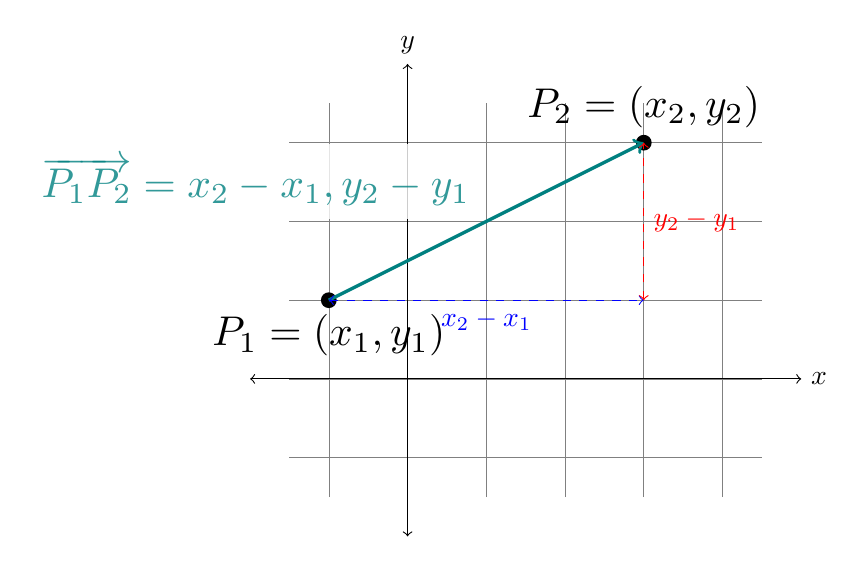
\begin{tikzpicture}
\draw[gray, very thin] (-1.5,-1.5) grid (4.5,3.5);
\draw[<->] (-2,0) -- (5,0) node [pos=1, right] {$x$};
\draw[<->] (0,-2) -- (0,4) node [pos=1, above] {$y$};
\fill (-1,1) circle [radius = 0.1cm] node [scale = 1.5, below] {$P_1 = (x_1, y_1)$};
\fill (3,3) circle [radius = 0.1cm] node [scale = 1.5, above] {$P_2 = (x_2, y_2)$};
\draw[->, very thick, teal] (-1,1) -- (3,3) node [fill = white, fill opacity = 0.8, pos=0.5, above left, scale = 1.5] {$\overrightarrow{P_1P_2} = \bv{ x_2 - x_1, y_2 - y_1}$};
\draw[dashed, <->, blue] (-1,1) -- (3,1) node [below, pos =0.5] {$x_2-x_1$};
\draw[dashed, <->, red] (3,1) -- (3,3) node [right, pos=0.5] {$y_2-y_1$};
\end{tikzpicture}
\caption{เวกเตอร์ที่เริ่มต้นที่จุด $P_1$ ไปยังจุด $P_2$}
\end{figure}
\end{frame}


\begin{frame}[t]
\begin{ex}{}
จงหาเวกเตอร์จากจุดต่อไปนี้
\begin{tasks}(2)
\task $P_1(3,2)$ ไปยังจุด $P_2(4,6)$
\task $Q_1(-1,0)$ ไปยังจุด $Q_2(3,-2)$
\end{tasks}
\end{ex}
\begin{sol}
เราใช้สูตรคำนวณได้โดยตรง \pa เป็น
\begin{tasks}(1)
\task $\overrightarrow{P_1P_2} \pa = \bv{4-3, 6-2} \pa = \bv{1,4}$ \pa
\task $\overrightarrow{Q_1Q_2} \pa = \bv{3-(-1), -2-0} \pa = \bv{4,-2}$
\end{tasks}
\end{sol}
\end{frame}

\begin{frame}
\frametitle{หลักเกณฑ์ทางเลขคณิตของเวกเตอร์}
\begin{prop}{}{}
กำหนดเวกเตอร์ $\vec{u}, \vec{v}$ และค่าคงตัว $k,l$ แล้ว
\begin{enumerate}
\item $\vec{u} + \vec{v} = \vec{v} + \vec{u}$ (สมบัติการสลับที่) \pa
\item $(\vec{u} + \vec{v}) + \vec{w} = \vec{u} + (\vec{v} + \vec{w})$ (สมบัติการเปลี่ยนกลุม่) \pa
\item $\vec{u} + \vec{0} = \vec{0} + \vec{u} = \vec{u}$ \pa เมื่อ $\vec{0} = \bv{0,0}$ ในปริภูมิสองมิติ และ $\vec{0} = \bv{0,0,0}$ ในปริภูมิสามมิติ
\item $\vec{u} + (-\vec{u}) = \vec{0}$ \pa
\item $k(l \vec{u}) = (kl) \vec{u}$ \pa
\item $k(\vec{u} + \vec{v}) = k\vec{u} + k\vec{v}$ (สมบัติการกระจาย)
\end{enumerate}
\end{prop}
\end{frame}


%%%%%%%%%%%%%
\section{ขนาดของเวกเตอร์}
\frame{\sectionpage}
%%%%%%%%%%%%%

\begin{frame}
\frametitle{ขนาดของเวกเตอร์}
\begin{defn}{}{}
กำหนดเวกเตอร์ $\vec{v}$ แล้ว\alert{ขนาดของเวกเตอร์  $\vec{v}$} เขียนแทนด้วย $\| \vec{v} \|$ คือระยะทางจากจุดเริ่มต้นไปจุดสิ้นสุดของเวกเตอร์ \pa

ถ้า $\vec{v} = \langle v_1, v_2 \rangle $ แล้ว 
\begin{equation}
\| \vec{v} \| = \sqrt{v_1^2 + v_2^2}
\end{equation} \pa

ถ้า $\vec{v} = \langle v_1, v_2, v_3\rangle$ แล้ว 
\begin{equation}
\| \vec{v} \| = \sqrt{v_1^2 + v_2^2 + v_3^2}
\end{equation} \pa
\end{defn}
\end{frame}

\begin{frame}
\begin{figure}[h!]
\centering
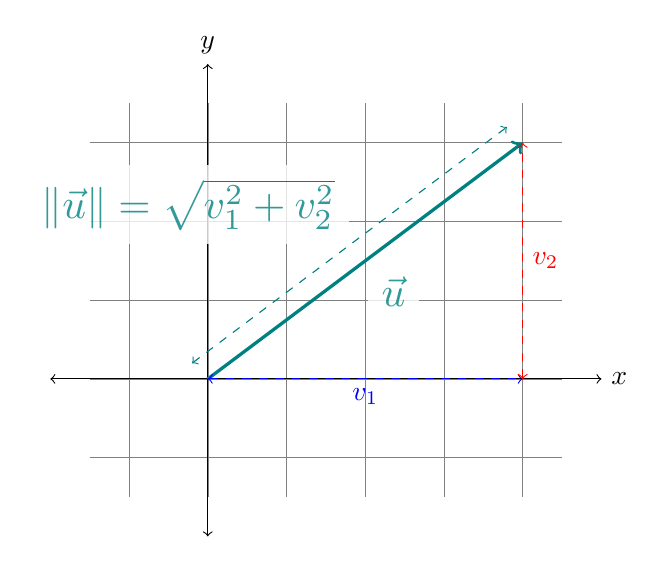
\begin{tikzpicture}
\draw[gray, very thin] (-1.5,-1.5) grid (4.5,3.5);
\draw[<->] (-2,0) -- (5,0) node [pos=1, right] {$x$};
\draw[<->] (0,-2) -- (0,4) node [pos=1, above] {$y$};
\draw[->, very thick, teal] (0,0) -- (4,3) node [fill = white, fill opacity = 0.8, pos=0.5, below right, scale = 1.5] {$\vec{u}$};
\draw[<->, dashed, teal] (-0.2,0.2) -- (3.8,3.2) node [fill = white, fill opacity = 0.8, pos=0.5, above left, scale = 1.5] {$\| \vec{u} \| = \sqrt{v_1^2 + v_2^2}$};
\draw[<->, dashed, blue] (0,0) -- (4,0) node [below, pos =0.5] {$v_1$};
\draw[<->, dashed, red] (4,0) -- (4,3) node [right, pos=0.5] {$v_2$};
\end{tikzpicture}
\caption{ขนาดของเวกเตอร์ $\vec{u}$}
\end{figure}
\end{frame}



\begin{frame}[t]
\begin{ex}{}
จงหาขนาดของเวกเตอร์ต่อไปนี้
\begin{tasks}(2)
\task $\bv{3,4}$
\task $\bv{0,3}$
\task $\bv{2,-2,1}$
\task $\bv{1,2,3}$
\end{tasks}
\end{ex}
\begin{sol}
\begin{tasks}(1)
\task $\| \bv{3,4} \| \pa = \sqrt{3^2+4^2} \pa = \sqrt{25} \pa = 5$ \pa
\task $\| \bv{0,3} \| \pa = \sqrt{0^2 + 3^2} \pa = \sqrt{9}\pa = 3$ \pa
\task $\| \bv{2,-2,1} \| \pa = \sqrt{2^2 + (-2)^2 + 1^2} \pa = \sqrt{9} = 3$ \pa
\task $\| \bv{1,2,3} \| \pa = \sqrt{1^2 + 2^2 + 3^2} \pa = \sqrt{14}$
\end{tasks}
\end{sol}
\end{frame}

\begin{frame}
\frametitle{สมบัติของขนาดเวกเตอร์}
\begin{prop}{}{}
กำหนดให้ $\vec{u}$ เป็นเวกเตอร์ในปริภูมิสองมิติ หรือเวกเตอร์ในปริภูมิสามมิติ
\begin{enumerate}
\item $\| \vec{u} \| \geq 0$ (ขนาดไม่มีทางติดลบ)\pa
\item $\| \vec{u} \| = 0$ ก็ต่อเมื่อ $\vec{u}$ คือเวกเตอร์ศูนย์ ($\bv{0,0}$ ในปริภูมิสองมิติ และ $\bv{0,0,0}$ ในปริภูมิสามมิติ) \pa
\item $\| k \vec{u} \| = |k| \times \|\vec{u}\|$ (ถ้าคูณเวกเตอร์ด้วยค่าคงตัว $k$ แล้วขนาดจะเพิ่มเป็น $|k|$ เท่า) \pa
\item ถ้า $\vec{u}, \vec{v}$ เป็นเวกเตอร์ที่ทำมุม $\theta$ ระหว่างกันแล้ว 
\begin{equation}
\| \vec{u} + \vec{v} \|^2 = \| \vec{u} \|^2 + \|\vec{v}\|^2 + 2\| \vec{u} \|\|\vec{v}\| \cos \theta
\end{equation}
\end{enumerate}

\end{prop}
\end{frame}


%%%%%%%%%%%%%
\section{เวกเตอร์หนึ่งหน่วย}
\frame{\sectionpage}
%%%%%%%%%%%%%

\begin{frame}[t]
\frametitle{เวกเตอร์หนึ่งหน่วย}
\begin{defn}{}{}
เวกเตอร์หนึ่งหน่วย (Unit vector) คือ เวกเตอร์ที่มีขนาดเท่ากับ 1
\end{defn}\pa

\begin{figure}[h!]
\centering
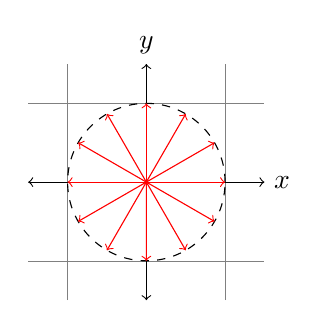
\begin{tikzpicture}
\draw[gray, very thin] (-1.5,-1.5) grid (1.5,1.5);
\draw[<->] (-1.5,0) -- (1.5,0) node [pos=1, right] {$x$};
\draw[<->] (0,-1.5) -- (0,1.5) node [pos=1, above] {$y$};
\draw[dashed] (0,0) circle [radius = 1cm];
\foreach \r in {0,1,...,11}
{
	\draw[->, red] (0,0) -- (\r*pi/6 r: 1cm);
}
\end{tikzpicture}
\caption{ตัวอย่างเวกเตอร์หนึ่งหน่วย}
\end{figure}
\end{frame}

\begin{frame}
\frametitle{เวกเตอร์หน่วยทิศทางขนานกับแกน}
\begin{defn}{}{}
ในปริภูมิสองมิติ นิยามเวกเตอร์หนึ่งหน่วยในทิศทางขนานกับแกน $x$ และแกน $y$ ดังนี้\pa
\[\bvec{i} = \vec{i} = \bv{1,0} \pa, \qquad \bvec{j} = \vec{j} = \bv{0,1}\]
ในปริภูมิสามมิติ นิยามเวกเตอร์หนึ่งหน่วยในทิศทางขนานกับแกน $x$ แกน $y$ และแกน $z$ ดังนี้\pa
\[\bvec{i} = \vec{i} = \bv{1,0,0} \pa \qquad  \bvec{j} = \vec{j} = \bv{ 0,1,0 } \pa \qquad \bvec{k} = \vec{k} = \bv{ 0,0,1} \]
\end{defn} \pa
ในเอกสารนี้ เราจะใช้ $\vec{i}, \vec{j}$ และ $\vec{k}$ 
\end{frame}


\begin{frame}
\begin{figure}[h!]
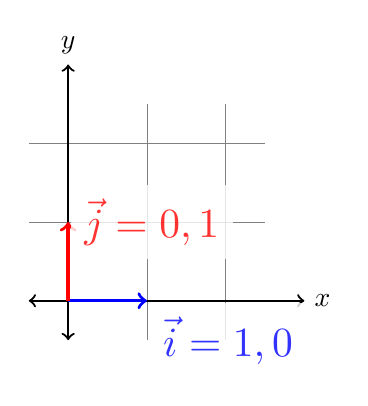
\begin{tikzpicture}
\draw[very thin,color=gray] (-0.5,-0.5) grid (2.5,2.5);
\draw[<->, thick] (-0.5,0) -- (3,0) node[right] {$x$};
\draw[<->, thick] (0,-0.5) -- (0,3) node[above] {$y$};
\draw[->, blue, very thick] (0,0) -- (1,0) node[below right, scale = 1.5, fill = white, fill opacity = 0.8] {$\vec{i} = \bv{1,0}$};
\draw[->, red, very thick] (0,0) -- (0,1) node[right, scale = 1.5, fill = white, fill opacity = 0.8] {$\vec{j} = \bv{0,1}$};
\end{tikzpicture}
\caption{เวกเตอร์หน่วย $\vec{i}$ และ $\vec{j}$}
\end{figure}

\begin{slide}
เราสามารถเขียน $\vec{v}$ ในปริภูมิสองมิติ ในรูปของเวกเตอร์หนึ่งหน่วย $\vec{i}$ และ $\vec{j}$ ได้ดังนี้
\[ \vec{v} = \bv{v_1, v_2} \pa = \vv{v_1}{+ v_2}\]
\end{slide}
\end{frame}

\begin{frame}
\begin{figure}[h!]
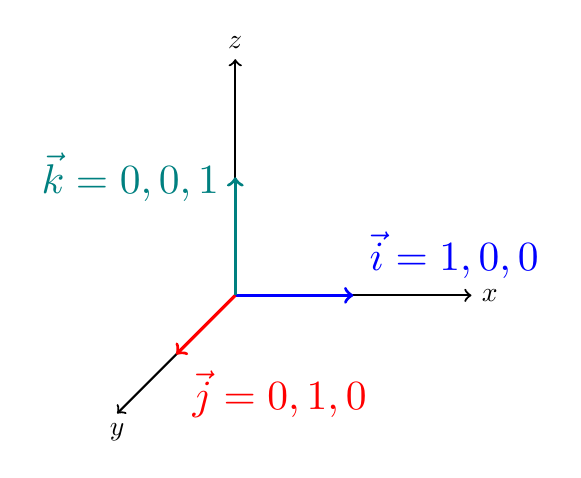
\begin{tikzpicture}[scale = 1.5]
\draw[->, thick] (0,0) -- (2,0) node[right] {$x$};
\draw[->, thick] (0,0) -- (-1,-1) node[left, below] {$y$};
\draw[->, thick] (0,0) -- (0,2) node[above] {$z$};
\draw[->, blue, very thick] (0,0) -- (1,0) node[above right, scale = 1.5] {$\vec{i} = \bv{1,0,0}$};
\draw[->, red, very thick] (0,0) -- (-0.5,-0.5) node[below right, scale = 1.5] {$\vec{j} = \bv{0,1,0}$};
\draw[->, teal, very thick] (0,0) -- (0,1) node[left, scale = 1.5] {$\vec{k} = \bv{0,0,1}$};
\end{tikzpicture}
\caption{เวกเตอร์หน่วย $\vec{i}, \vec{j}$ และ $\vec{k}$}
\end{figure}

\begin{slide}
เราสามารถเขียน $\vec{v}$ ในปริภูมิสามมิติ ในรูปของเวกเตอร์หน่วย $\vec{i}, \vec{j}$ และ $\vec{k}$ ได้ดังนี้
\[ \vec{v} = \bv{v_1, v_2, v_3} \pa = \vvv{v_1}{+ v_2}{+ v_3}\]
\end{slide}
\end{frame}


\begin{frame}[t]
\begin{ex}{}
จงแปลงเวกเตอร์ต่อไปนี้ให้เป็นรูปของเวกเตอร์หนึ่งหน่วย $\vec{i}$ และ $\vec{j}$ 
\begin{tasks}(2)
\task $\bv{3,4} $
\task $\bv{-2,2}$
\task $\bv{2,-2,1}$
\task $\bv{0,0,1}$
\end{tasks}
\end{ex}
\begin{sol}
\begin{tasks}(1)
\task $\bv{3,4} \pa = \vv{3}{+4}$ \pa
\task $\bv{-2,2} \pa= \vv{-2}{+2}$ \pa
\task $\bv{2,-2,1} \pa= \vvv{2}{-2}{+}$ \pa
\task $\bv{0,0,1} \pa = \vvv{0}{+0}{+} \pa = \bvec{k}$
\end{tasks}
\end{sol}
\end{frame}


\begin{frame}[t]
\begin{ex}{}
จงแปลงเวกเตอร์ต่อไปนี้ให้เป็นรูปของเวกเตอร์ $\langle , \rangle$
\begin{tasks}(2)
\task $\vv{2}{-5} $
\task $3\bvec{i}$
\task $\vvv{2}{-2}{+1}$
\task $\bvec{j} - 2\bvec{k}$
\end{tasks}
\end{ex}
\begin{sol}
\begin{tasks}(1)
\task $\vv{2}{-5} \pa = \bv{2,-5}$ \pa
\task $3\bvec{i} \pa = 3\bvec{i} + 0\bvec{j} \pa = \bv{3,0}$ \pa
\task $\vvv{2}{-2}{+} \pa = \bv{2,-2,1}$ \pa
\task $\bvec{j} - 2\bvec{k} \pa = 0\bvec{i} + \bvec{j} - 2\bvec{k} \pa = \bv{0,1,-2}$
\end{tasks}
\end{sol}
\end{frame}

\begin{frame}[t]
\frametitle{เวกเตอร์หนึ่งหน่วยที่มีทิศทางเดียวกันกับ $\vec{u}$}
\begin{defn}{}{}
กำหนดเวกเตอร์ $\vec{u}$ แล้ว\alert{เวกเตอร์หนึ่งหน่วยที่มีทิศทางเดียวกันกับ $\vec{u}$} คือ $\frac{1}{\| \vec{u} \|} \vec{u} $
\end{defn}

\begin{figure}[h!]
\centering
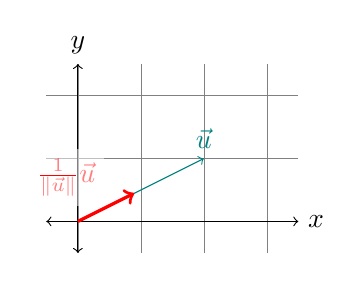
\begin{tikzpicture}[scale=0.8]
\draw[gray, very thin] (-0.5,-0.5) grid (3.5,2.5);
\draw[<->] (-0.5,0) -- (3.5,0) node [pos=1, right] {$x$};
\draw[<->] (0,-0.5) -- (0,2.5) node [pos=1, above] {$y$};
\draw[->, teal] (0,0) -- (2,1) node [pos=1, above] {$\vec{u}$};
\draw[->, very thick, red] (0,0) -- (0.894,0.447) node [pos = 0.5, above left, fill = white, fill opacity = 0.5] {$\frac{1}{\| \vec{u} \|} \vec{u}$};
\end{tikzpicture}
\caption{เวกเตอร์หนึ่งหน่วยที่มีทิศทางเดียวกันกับ $\vec{u}$}
\end{figure}
\end{frame}


\begin{frame}[t]
\begin{ex}
จงหาเวกเตอร์หนึ่งหน่วยที่มีทิศทางเดียวกันกับเวกเตอร์ $\bv{3,4}$
\end{ex}
\begin{sol}
$$\| \bv{3,4} \| \pa = \sqrt{3^2+4^2} = 5$$ \pa
ดังนั้นเวกเตอร์หนึ่งหน่วยที่มีทิศทางเดียวกันคือ \pa
\begin{eq*}
\frac{1}{5} \bv{3,4} \pa &=& \bv{ \frac{1}{5} \times 3, \frac{1}{5} \times 4 } \pa \\
&=& \bv{\frac{3}{5}, \frac{4}{5}}
\end{eq*}
\end{sol}
\end{frame}


\begin{frame}[t]
\begin{ex}
จงหาเวกเตอร์หนึ่งหน่วยที่มีทิศทางเดียวกันกับเวกเตอร์ $\bv{2,-2,1}$
\end{ex}
\begin{sol}
$$\| \bv{2,-2,1} \| \pa = \sqrt{2^2+(-2)^2+1^2} = 3$$ \pa
ดังนั้นเวกเตอร์หนึ่งหน่วยที่มีทิศทางเดียวกันคือ \pa
\begin{eq*}
\frac{1}{3} \bv{2,-2,1} \pa &=& \bv{ \frac{1}{3} \times 2, \frac{1}{3} \times (-2), \frac{1}{3} \times 1 } \pa \\
&=& \bv{\frac{2}{3}, \frac{-2}{3}, \frac{1}{3}}
\end{eq*}
\end{sol}
\end{frame}


%%%%%%%%%%%%%
\section{ผลคูณจุด}
\frame{\sectionpage}
%%%%%%%%%%%%%

\begin{frame}
\frametitle{นิยามผลคูณจุด}
\begin{defn}{}{}
กำหนดให้ $\vec{u} = \langle u_1, u_2 \rangle$ และ $\vec{v} = \langle v_1, v_2 \rangle$ เป็นเวกเตอร์ 2 มิติ \pa แล้ว\alert{ผลคูณจุด}ของเวกเตอร์ทั้งสองคือ $\vec{u} \cdot \vec{v}$ ซึ่งเป็นปริมาณสเกลาร์ที่นิยามด้วย

\begin{equation}
\vec{u} \cdot \vec{v} \pa = u_1v_1 + u_2v_2
\end{equation} \pa

กำหนดให้ $\vec{u} = \langle u_1, u_2, u_3 \rangle$ และ $\vec{v} = \langle v_1, v_2, v_3 \rangle$ เป็นเวกเตอร์ 3 มิติ \pa แล้ว\alert{ผลคูณจุด}ของเวกเตอร์ทั้งสองคือ $\vec{u} \cdot \vec{v}$ ซึ่งเป็นปริมาณสเกลาร์ที่นิยามด้วย

\begin{equation}
\vec{u} \cdot \vec{v} \pa = u_1v_1 + u_2v_2 + u_3v_3
\end{equation}
\end{defn}
\end{frame}


\begin{frame}[t]
\begin{ex}{}
จงหาผลคูณจุดของเวกเตอร์ต่อไปนี้
\begin{tasks}(2)
\task $\bv{3,4} \cdot \bv{1,2}$
\task $\bv{-2,2} \cdot \bv{-2,1}$
\task $\bv{0,3} \cdot \bv{9,0}$
\task $\bv{2,-2,1} \cdot \bv{1,1,3}$
\end{tasks}
\end{ex}
\begin{sol}
\begin{tasks}(1)
\task $\bv{3,4} \cdot \bv{1,2} \pa = (3 \times 1) \pa + (4 \times 2) \pa = 3 + 8 \pa = 11$ \pa
\task $\bv{-2,2} \cdot \bv{-2,1} \pa = ((-2) \times (-2)) \pa + (2 \times 1) \pa = 4 + 2 \pa = 6$ \pa
\task  $\bv{0,3} \cdot \bv{9,0} \pa = (0 \times 9) + (3 \times 0) \pa = 0 + 0 \pa = 0$ \pa
\task $\bv{2,-2,1} \cdot \bv{1,1,3} \pa = (2 \times 1) \pa + ((-2) \times 1) \pa + (1 \times 3) \pa = 2 + (-2) + 3 \pa = 3$
\end{tasks}
\end{sol}
\end{frame}

\begin{frame}
\frametitle{สมบัติของผลคูณจุด}
\begin{prop}{สมบัติของผลคูณจุด}{}
\begin{enumerate}
\item $\vec{u} \cdot \vec{v} = \vec{v} \cdot \vec{u}$ \pa
\item $\vec{u} \cdot (\vec{v} + \vec{w}) =  \vec{u} \cdot \vec{v}  + \vec{u} \cdot \vec{w}$ \pa
\item $k(\vec{u} \cdot \vec{v} ) = (k\vec{u}) \cdot \vec{v} = \vec{u} \cdot (k \vec{v})$ \pa
\item $\vec{u} \cdot \vec{u} = \| \vec{u} \|^2$ \pa
\item $\vec{0} \cdot \vec{u} = 0$ \pa
\item $\vec{u} \cdot \vec{v} = \| \vec{u} \| \|\vec{v} \| \cos \theta$ เมื่อ $\theta$ คือมุมระหว่างเวกเตอร์ $\vec{u}$ และ $\vec{v}$
\end{enumerate}
\end{prop}
\end{frame}
